\section{Verbraucher bei Gleich- und Wechselstrom} 

% TODO
Dieser Teilversuch beschäftigt sich mit der Untersuchung des Verhaltens von verschiedenen Verbrauchern bei Gleich- und Wechselstrom.
Dazu werden verschiedene Verbraucher an einen Stromkreis geschlossen, in dem je nach Einstellung ein Gleich- bzw. Wechselstrom fließt.
Es werden die bei den verschieden Strömen erhaltenen Spannungen, Stromstärken und Leistungen verglichen und Beziehungen mit der Theorie, insbesondere der Impedanzen für die Spule und den Kondensator behandelt. 
Die Theorie zu bestätigen ist das Ziel dieses Versuches.
%Die Ergebnisse werden kurz, aber mit konkreten Werten erwähnt.
%Dann werden diese in den Kontext kurz eingebunden.

\subsection{Methoden}

\subsubsection{Aufbau}

Der Aufbau des Versuches ist in Abb. \ref{fig:Schaltskizze} dargestellt\footnote{Die Schaltskizze wurde der Versuchsanleitung entnommen.}.
Dieser besteht aus einem Schaltkreis, in dem sich die Spannungsquelle, ein regulierbarer Widerstand  $R_1$ mit bis zu \SI{27}{\Omega}, sowie Messgeräte für den Leistungsverbrauch, die Spannung und den elektrischen Strom befinden. 
Die Spannungsquelle liefert nach ihrer Angabe \SI{24}{\V}. Gleich- und Wechselstrom sind hierbei beliebig einstellbar.
\begin{figure}[ht]
	\centering
	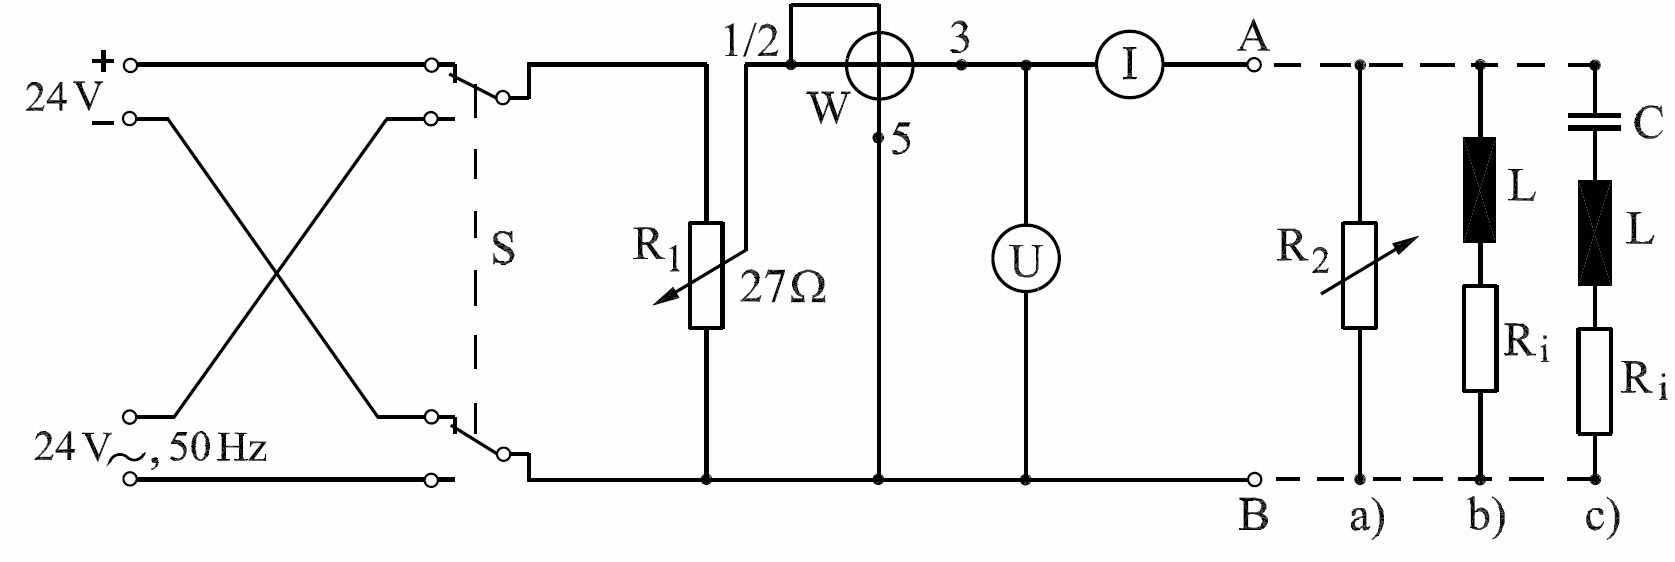
\includegraphics[width=0.9\textwidth]{auswertung/Schaltung2.png}
	\caption{Diese Schaltskizze stellt den Aufbau des Versuchs dar. Eingezeichnet sind die verschiedenen Verbraucher a), b) und c), welche in dem Versuch betrachtet werden.}
	\label{fig:Schaltskizze}	
\end{figure}
Zunächst wird die Leistung ohne angeschlossenen Verbraucher, also die Verlustleistung, für Gleich- und Wechselstrom gemessen. 
Dann werden verschiedene Verbraucher angeschlossen und für diese die Leistung, die Spannung und der elektrische Strom gemessen.
Auch dies erfolgt für Gleich- und Wechselstrom.
Bei den verwendeten Verbrauchern handelt es sich um einen Widerstand $R_2$, dann um eine Spule $L$ mit Innenwiderstand $R_i$ und zuletzt um dieselbe Spule, jedoch mit zusätzlich angeschlossenem Kondensator.
Für den letzten Fall wird nur bei Wechselstrom gemessen, da bei diesem Fall zusätzliche Effekte zum Tragen kommen.

\subsubsection{Unsicherheiten}

Die bei der Aufnahme der Messwerte zu berücksichtigenden Unsicherheiten treten hier bei den Angaben der Spannungsquelle, der Widerstände, des Kondensators, sowie bei dem Ablesen von den Messgeräten auf. 
Da es sich bei letzteren immer um Analoganzeigen gehandelt hat, wird die Unsicherheit dieser durch eine Dreiecksverteilung abhängig von der Genauigkeit der Skala bestimmt. 
Ansonsten werden die angegebenen Unsicherheiten verwendet, welche alle bei 10\% des dargestellten Werts liegen. Für die Spannungsquelle gab es keine Angabe, weswegen auch hier mit 10\% der angegebenen \SI{24}{\V} gerechnet werden.
Im Allgemeinen werden zur Berechnung der kombinierten Unsicherheiten die nach GUM vorgesehenen Formeln verwendet. 
Die Berechnung dieser für diesen Versuch erfolgt im Anhang (\ref*{sec:anhang}).

\subsubsection{Komplikationen}

Trotz Korrektheit der Schaltung, welche von der Betreuerin geprüft wurde, konnten keine Werte gemessen werden. 
Der Austausch des Gerätes zur Messung der Leistung löste dieses Problem.
Allerdings war es nicht möglich mit dem Multimeter, welches bereits bei den Akkumulatorzellen verwendet wurde, ohne angeschlossenen Verbraucher, eine Spannung und die zugehörige Verlustleistung zu messen.
Das Messgerät für die Leistung schlug in den negativen Bereich aus, was aus physikalischer Sicht unlogisch war.
Aus diesem Grund wurde statt des Multimeters ein einfaches Voltmeter angeschlossen.
Damit ließen sich Werte messen, jedoch auch eine Spannung von ca. \SI{25,5}{\V}, was mehr als der Eingangsspannung entsprechen würde. Da dieser Wert jedoch innerhalb der angenommenen 10\% Unsicherheit liegt, wird er akzeptiert.

\subsection{Datenanalyse}

Alle aufgenommenen Werte sind dem Laborbuch zu entnehmen. 
Darüber hinaus sind die Daten in den folgenden Diagrammen graphisch dargestellt.
\begin{figure}[ht]
	\centering	
	\begin{subfigure}{0.70\textwidth}
		\centering
		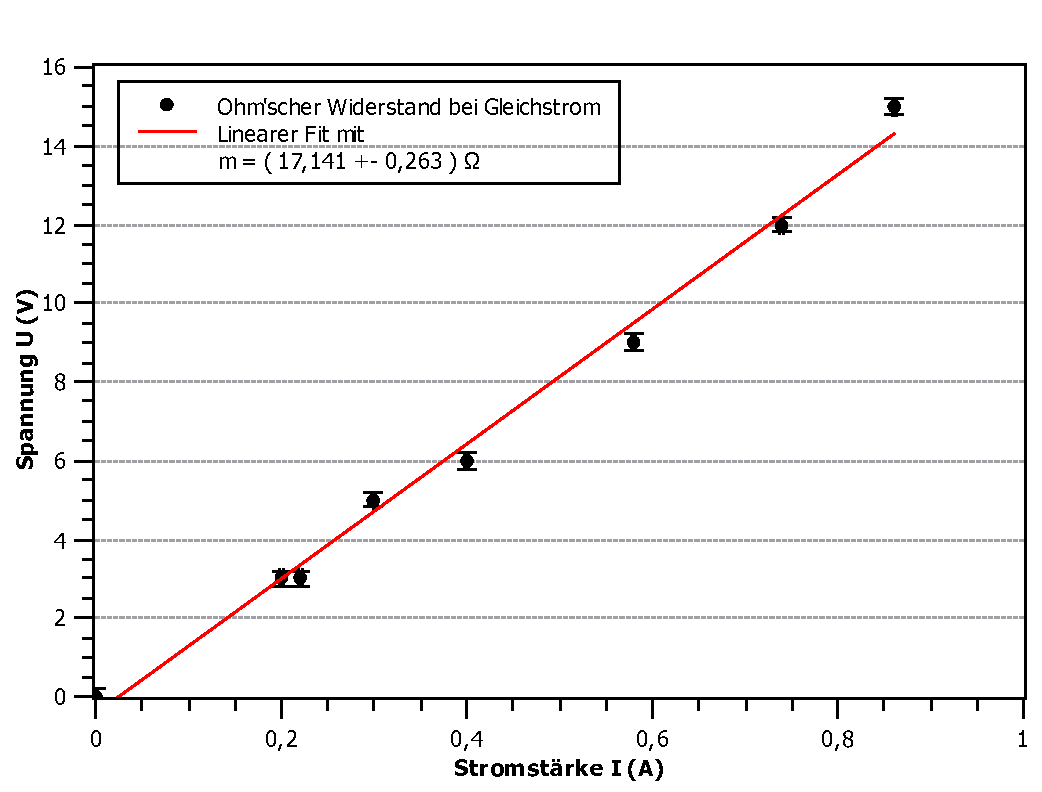
\includegraphics[width=\textwidth]{auswertung/widerstand_gleichstrom_Widerstand.pdf}
		\label{fig:1}
		\caption{Graphische Darstellungen der $U$-$I$-Kennlinie bei Gleichstrom und Widerstand als Verbraucher.}	
	\end{subfigure}
	\begin{subfigure}{0.70\textwidth}
		\centering
		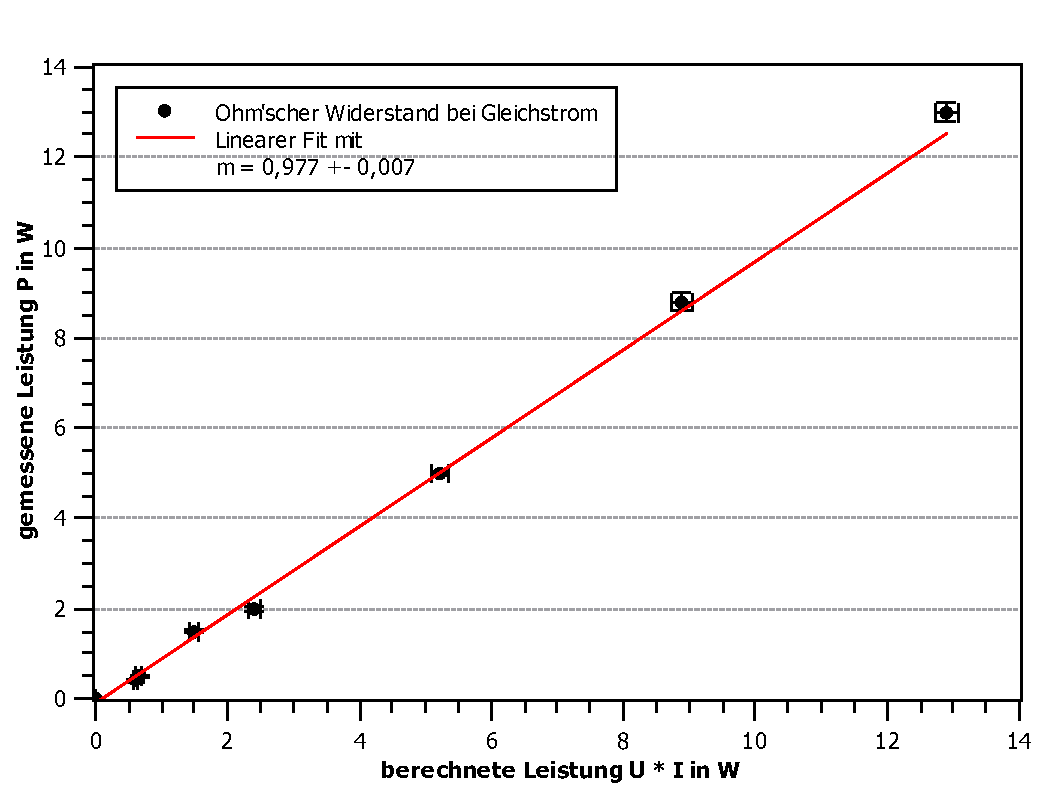
\includegraphics[width=\textwidth]{auswertung/widerstand_gleichstrom_Leistung.pdf}
		\label{fig:2}
		\caption{Verhältnis der ermittelten und gemessenen Leistung bei Gleichstrom und Widerstand als Verbraucher.}	
	\end{subfigure}
	\caption{Graphische Darstellungen der $U$-$I$-Kennlinie des Widerstands, sowie Verhältnis der ermittelten und gemessenen Leistung bei dem Widerstand als Verbraucher bei Gleichstrom.}
\end{figure}
\begin{figure}[ht]
	\centering	
	\begin{subfigure}{0.70\textwidth}
		\centering
		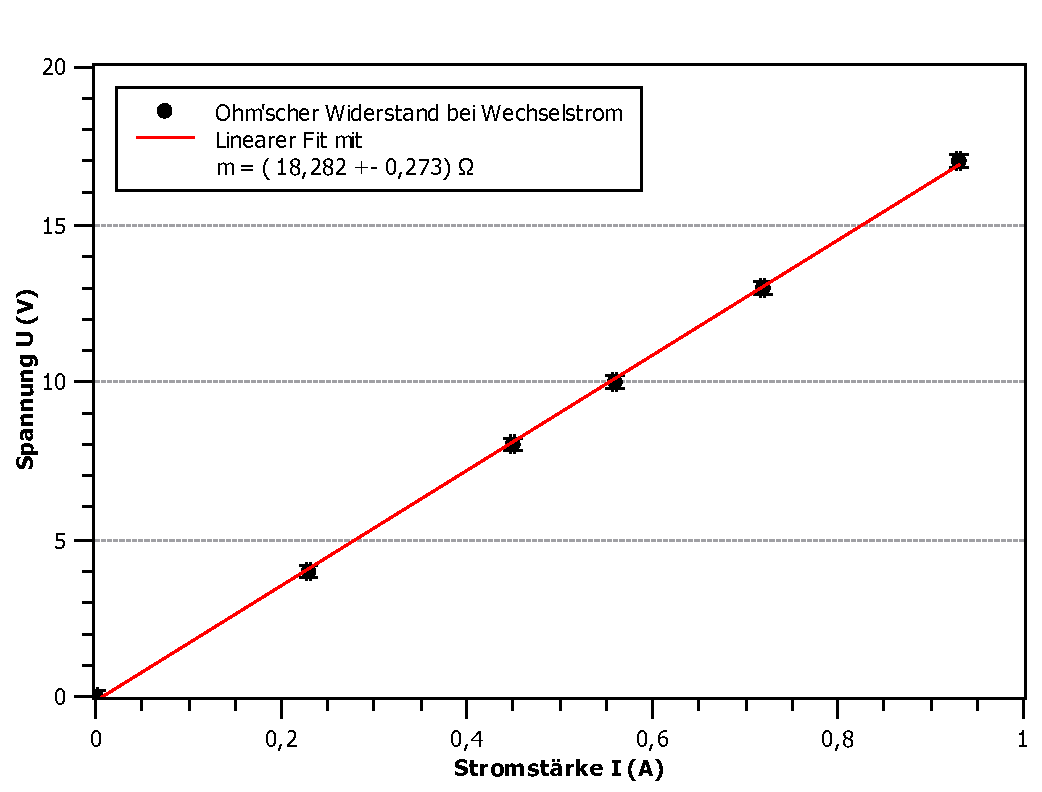
\includegraphics[width=\textwidth]{auswertung/widerstand_wechselstrom_Widerstand.pdf}
		\label{fig:3}
		\caption{Graphische Darstellungen der $U$-$I$-Kennlinie bei Wechselstrom und Widerstand als Verbraucher.}	
	\end{subfigure}
	\begin{subfigure}{0.70\textwidth}
		\centering
		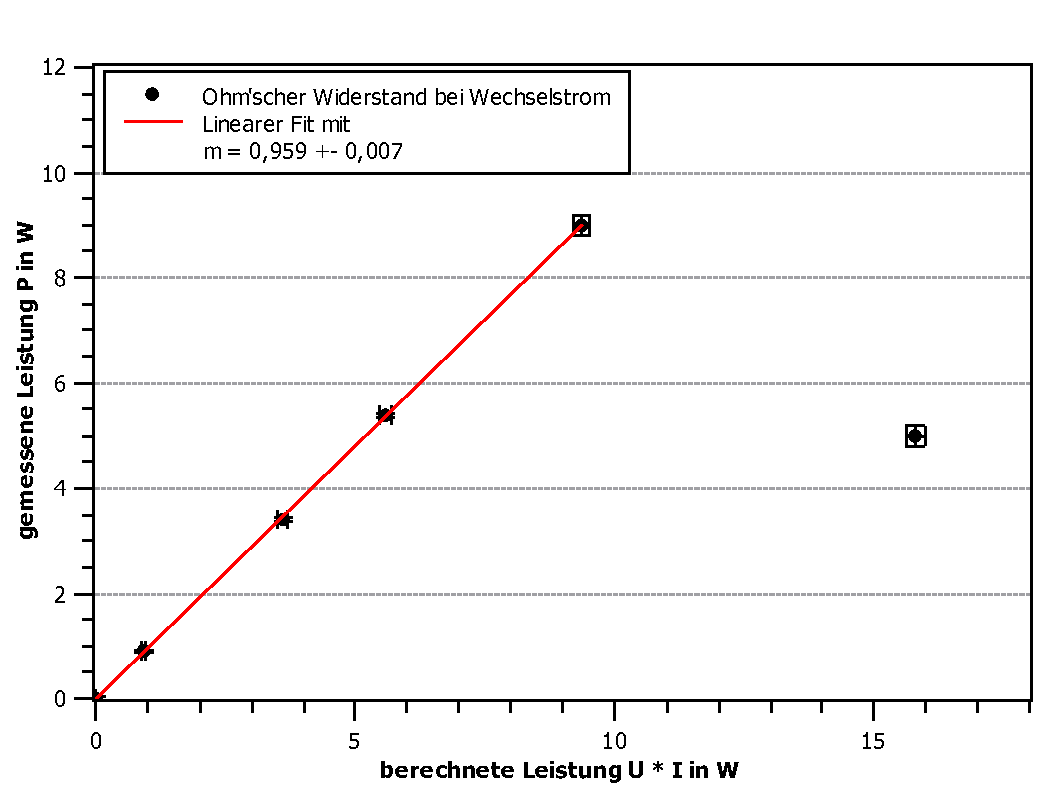
\includegraphics[width=\textwidth]{auswertung/widerstand_wechselstrom_Leistung.pdf}
		\label{fig:4}
		\caption{Verhältnis der ermittelten und gemessenen Leistung bei Wechselstrom und Widerstand als Verbraucher. Da der eine Messpunkt offensichtlich falsch aufgenommen wurde, wurde dieser nicht mit ausgewertet.}	
	\end{subfigure}
	\caption{Graphische Darstellungen der $U$-$I$-Kennlinie des Widerstands, sowie Verhältnis der ermittelten und gemessenen Leistung bei dem Widerstand als Verbraucher bei Wechselstrom.}
\end{figure}

\begin{figure}[ht]
	\centering	
	\begin{subfigure}{0.70\textwidth}
		\centering
		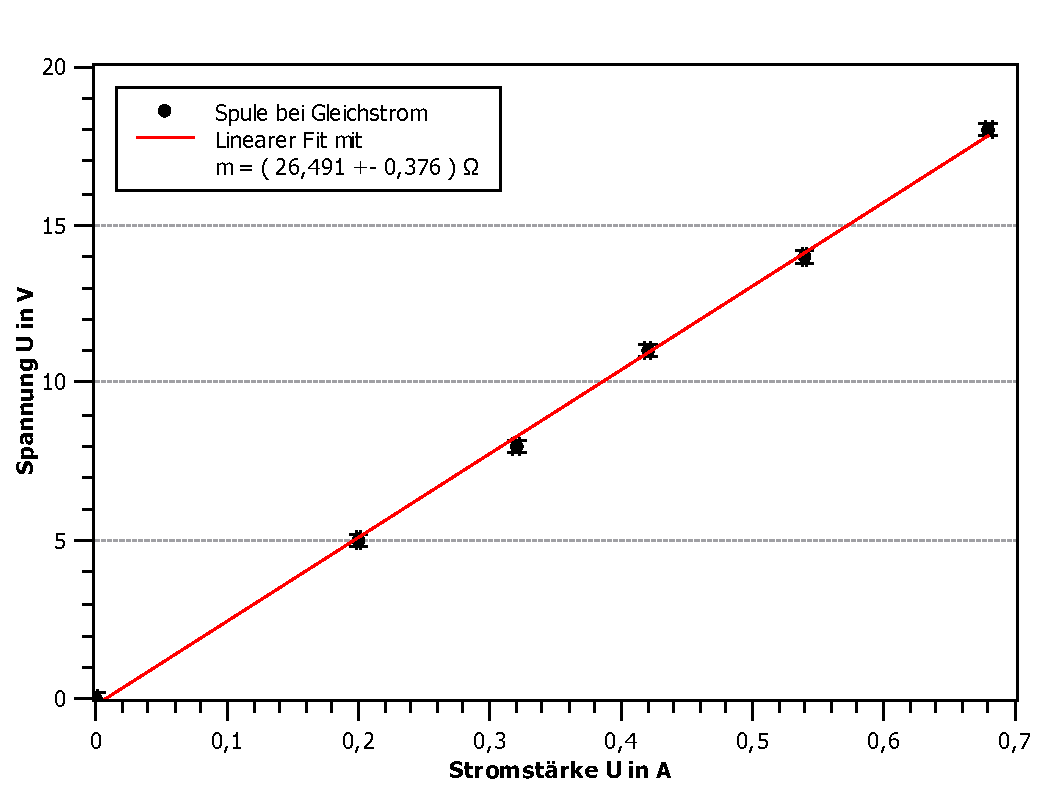
\includegraphics[width=\textwidth]{auswertung/spule-gleich-Widerstand.pdf}
		\label{fig:5}
		\caption{Graphische Darstellungen der $U$-$I$-Kennlinie bei Gleichstrom und Spule als Verbraucher.}	
	\end{subfigure}
	\begin{subfigure}{0.70\textwidth}
		\centering
		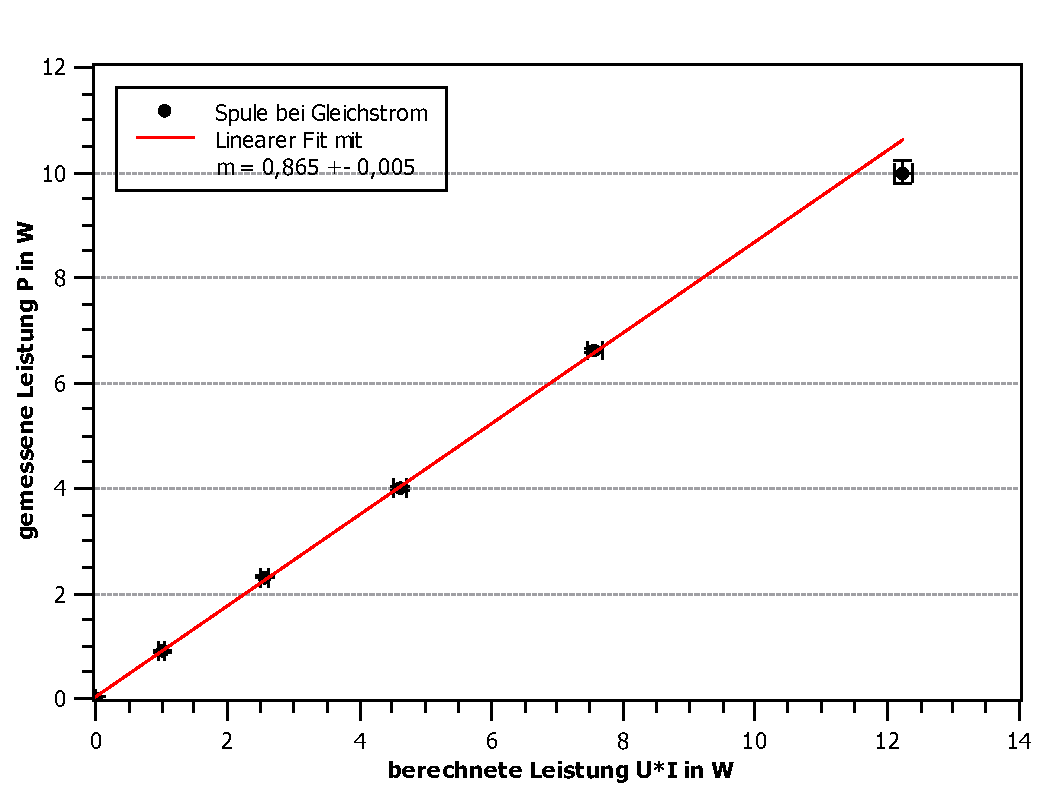
\includegraphics[width=\textwidth]{auswertung/spule-gleich-Leistung.pdf}
		\label{fig:6}
		\caption{Verhältnis der ermittelten und gemessenen Leistung bei Gleichstrom und Spule als Verbraucher.}	
	\end{subfigure}
	\caption{Graphische Darstellungen der $U$-$I$-Kennlinie des Widerstands, sowie Verhältnis der ermittelten und gemessenen Leistung bei der Spule als Verbraucher bei Gleichstrom.}
\end{figure}
\begin{figure}[ht]
	\centering	
	\begin{subfigure}{0.70\textwidth}
		\centering
		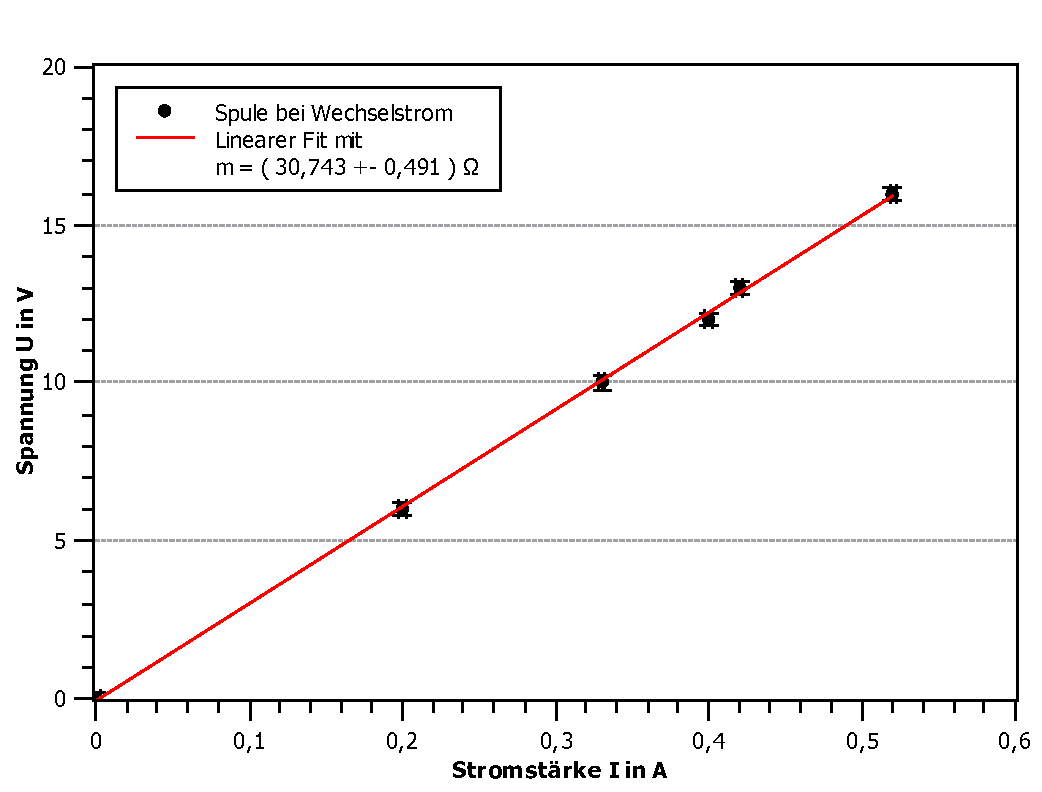
\includegraphics[width=\textwidth]{auswertung/spule-wechsel-Widerstand.pdf}
		\label{fig:7}
		\caption{Graphische Darstellungen der $U$-$I$-Kennlinie bei Wechselstrom und Spule als Verbraucher.}	
	\end{subfigure}
	\begin{subfigure}{0.70\textwidth}
		\centering
		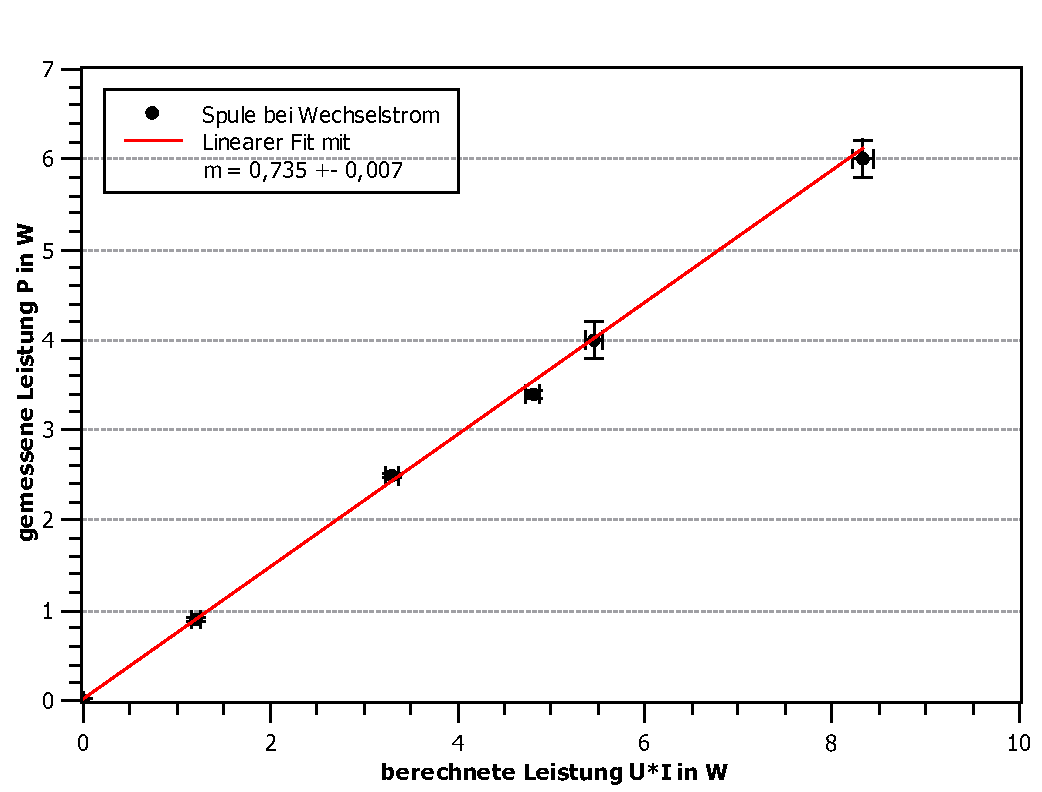
\includegraphics[width=\textwidth]{auswertung/spule-wechsel-Leistung.pdf}
		\label{fig:8}
		\caption{Verhältnis der ermittelten und gemessenen Leistung bei Wechselstrom und Spule als Verbraucher.}	
	\end{subfigure}
	\caption{Graphische Darstellungen der $U$-$I$-Kennlinie des Widerstands, sowie Verhältnis der ermittelten und gemessenen Leistung bei der Spule als Verbraucher bei Wechselstrom.}
\end{figure}

\begin{figure}[ht]
	\centering	
	\begin{subfigure}{0.70\textwidth}
		\centering
		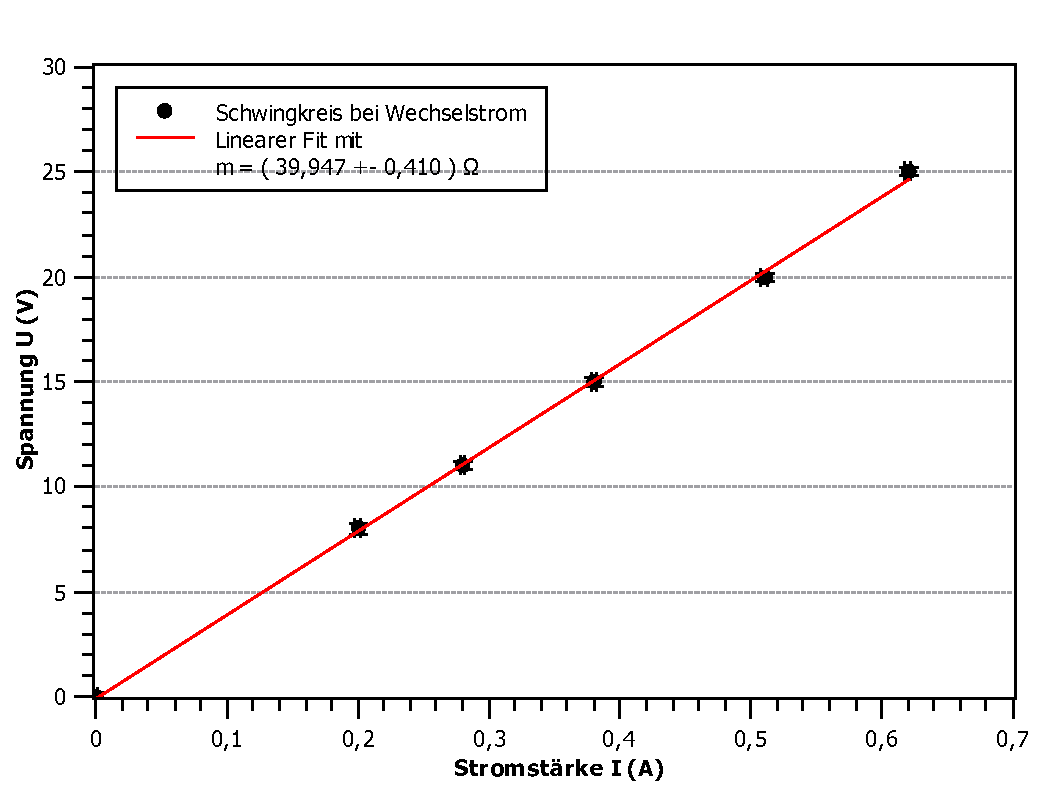
\includegraphics[width=\textwidth]{auswertung/kondensator-wechsel-Widerstand.pdf}
		\label{fig:9}
		\caption{Graphische Darstellungen der $U$-$I$-Kennlinie bei Wechselstrom und Kondensator und Spule als Verbraucher.}	
	\end{subfigure}
	\begin{subfigure}{0.70\textwidth}
		\centering
		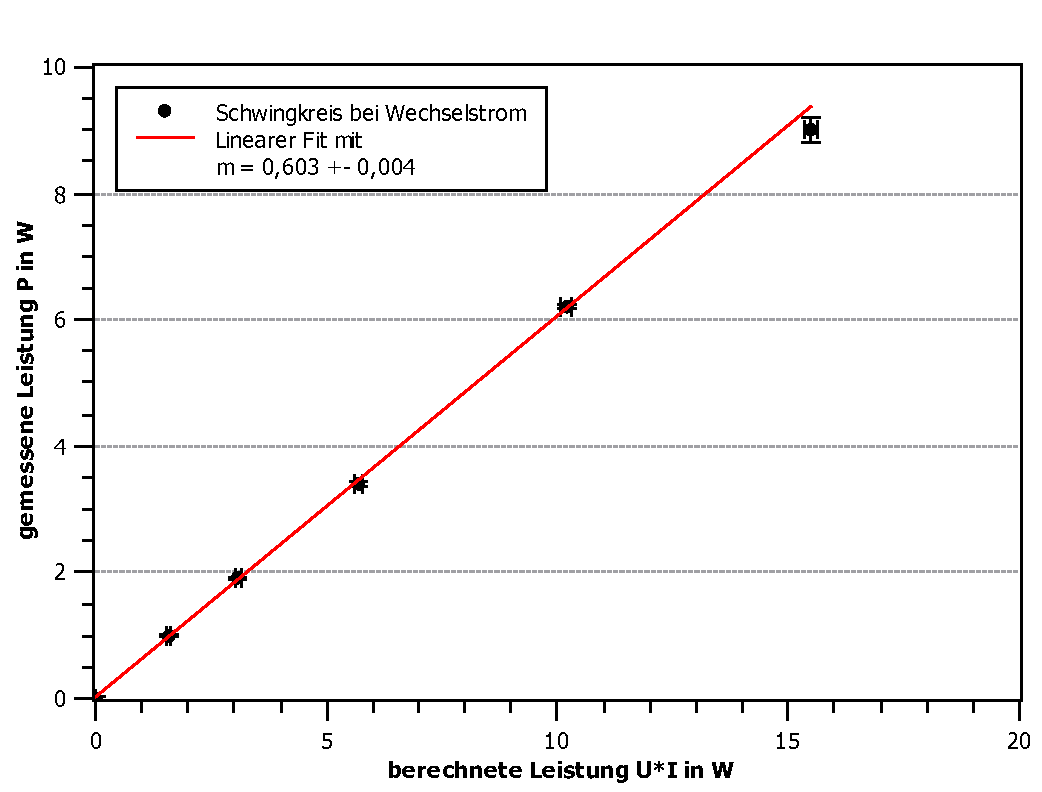
\includegraphics[width=\textwidth]{auswertung/kondensator-wechsel-Leistung.pdf}
		\label{fig:10}
		\caption{Verhältnis der ermittelten und gemessenen Leistung bei Wechselstrom und Kondensator und Spule als Verbraucher.}	
	\end{subfigure}
	\caption{Graphische Darstellungen der $U$-$I$-Kennlinie des Widerstands, sowie Verhältnis der ermittelten und gemessenen Leistung bei dem Kondensator und der Spule als Verbraucher bei Wechselstrom.}
\end{figure}

%Rechnungsweg zum Ergebnis angeben und begründen, warum z. B. linearer Fit genommen wurde.
%Dazu auf die Theorie oder die Versuchsanleitung Bezug nehmen.
%Vollständige Fehlerberechnung in den Anhang.
%Da grundsätzlich schon vorher erläutert (GUM) reicht hier eine kurze Anmerkung auf die Fehlerrechnung.
%Ergebnis graphisch darstellen und auf passende Darstellungsweise (Unsicherheiten, signifikante Stellen) achten.

%Falls mehrere voneinander unabhängige Lösungen existieren (z. B. bei der geometrischen Bestimmung des Trägheitsmomentes des Kreisels), können diese in Unterkapitel gegliedert werden.

\subsection{Diskussion}

%Die Ergebnisse in den Kontext einbinden.
%Zusammenhänge noch einmal darstellen.
%Jegliche Aussagen durch Ergebnisse oder Vorwissen untermauern.
%Ergebnisse mit Referenzwerten/Literaturwerten vergleichen und auf Unsicherheiten eingehen (Vertrauensgrad).

\subsection{Schlussfolgerung}

%Das Ziel noch einmal erläutern.
%Fazit des Versuchs angeben (untermauert die These; weicht von den Literaturwerten ab; ...).
%Warum folgt aus den Ergebnissen das Fazit.
%Mit ermittelten Daten und Unsicherheiten begründen.
%Auf Unsicherheiten weiter eingehen und Vertrauensgrad bzw. Relevanz der Schlussfolgerung auf die derzeitige Wissenslage angeben (meistens nicht relevant).
%Verbesserungsvorschläge für das nächste Mal und allgemeine Rekapitulierung über das durchgeführte Experiment.
%Warum muss man das Experiment unbedingt noch mal durchführen.
